\chapter{I primi modelli di Machine Learning}\label{chap:primi_modelli}

\section{Neurone computazionale - modello di McCulloch-Pitt}
L'idea iniziale era quella di replicare la struttura di un neurone biologico con un modello matematico, in modo da poter simulare il funzionamento del cervello umano. 

\paragraph{Neurone biologico.} Un neurone biologico è costituito da:
\begin{itemize}
	\item Dendriti: ricevono segnali da altri neuroni.
	\item Corpo cellulare: elabora i segnali ricevuti.
	\item Assone: trasmette il segnale elaborato ad altri neuroni.
\end{itemize}

\noindent
Il primo modello di neurone computazionale fu proposto da McCulloch e Pitts nel 1943. Si basa su tre componenti principali: 

\begin{itemize}
	\item Degli input $x_1, x_2, \dots, x_d$ binari, che possono essere \textbf{eccitatori }e \textbf{inibitori}. 
	\item Una threshold $v$, una soglia
	\item Un output binario.
\end{itemize}

\begin{figure}[tbph]
	\centering
	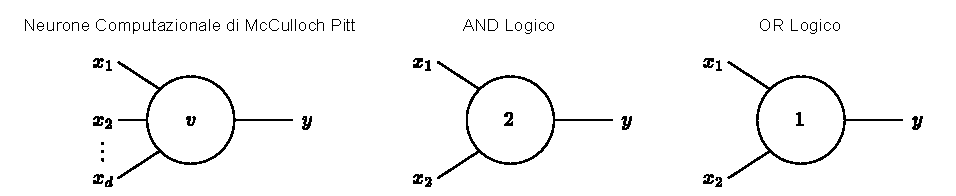
\includegraphics[width=\linewidth]{./images/neurone_computazionale.pdf}
	\caption{Modello di McCulloch Pitt e due computazioni possibili: AND logico e OR logico}
	\label{fig:neuronecomputazionale}
\end{figure}

Supponiamo che $x_1, \dots, x_j$ siano eccitatori, $x_{j+1}, \dots, x_d$ sono inibitori. Se $j \geq 1$ e almeno un inibitore è $=1$, allora il neurone ritorna 0. Un inibitore è sufficiente per bloccare l'output. Altrimenti, si calcola $z = x_1 + \dots + x_j = x_1 + \dots + x_d$, ossia la somma di tutti gli input\footnote{posso considerare anche gli input degli inibitori in quanto $=0$.}. Se la somma è $\geq v$, allora l'output sarà 1, altrimenti 0.

Questo modello è tale da poter computare un $AND$ ($v=n$ e $n$ input eccitatori), un $OR$ ($v=1$ e $n$ input eccitatori, vedere figura \ref{fig:neuronecomputazionale}), ma non uno $XOR$!

\subsection{Limitazioni del modello di McCulloch-Pitt}
\begin{itemize}
	\item Non esiste un modo automatico di fare training.
	\item Gli input sono binari.
	\item Gli input hanno tutti lo stesso peso.
	\item Tutte le funzioni computabili sono linearmente separabili.
\end{itemize}

\section{Percettrone - Rosenblatt}

Il successore del modello di McCulloch-Pitt è il \textbf{percettrone}. Questo modello risolve il problema dei pesi, assegnando ad ogni ingresso un peso differente, e introduce una procedura di apprendimento automatico per stabilire i pesi in maniera opportuna.
\begin{figure}[tbph]
	\centering
	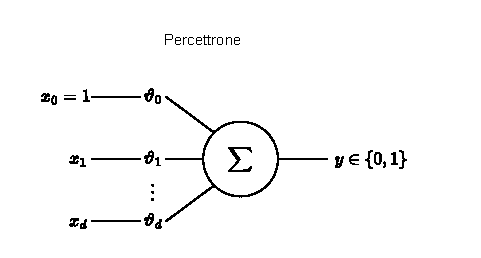
\includegraphics[width=\linewidth]{./images/percettrone.pdf}
	\caption{Modello di Rosenblatt, noto come Percettrone}
	\label{fig:percettrone}
\end{figure}

\noindent
Le componenti sono:
\begin{itemize}
	\item Features $x_1, x_2, \dots, x_d$ normalizzate in $[0, 1]$. Ciascuno di questi input ha associato un peso $\vartheta_1, \dots, \vartheta_d$.
	\item Una threshold $\vartheta_0$, una soglia.
	\item Un output binario.
	\item Una \textbf{procedura di learning automatico} per stabilire i parametri (il peso di ciascun input).
\end{itemize}

\noindent
Il comportamento del percettrone è il seguente:
\[
f(x_1,\dots,x_d)=
\begin{cases}
1 & se \displaystyle\sum_{j=0}^d \vartheta_j x_j \ge \vartheta_0\\
0 & \text{altrimenti.}
\end{cases}
\]

Per semplificare la notazione, introduciamo una feature \emph{dummy} $x_0=1$ e definiamo il vettore di input esteso
\[
\tilde{x}=(x_0,x_1,\dots,x_d)^\top,
\]
in modo da poter riscrivere la regola di decisione come una singola disuguaglianza. Per farlo, incorporiamo la soglia nella somma definendo un vettore di pesi esteso
\[
\vartheta=(\vartheta_0,\vartheta_1,\dots,\vartheta_d)^\top
\qquad\text{con}\qquad
\vartheta_0 = -\,\vartheta_0^{(\text{soglia})}.
\]
In questo modo otteniamo:
\[
f(x)=\mathbf{1}\{\vartheta^\top \tilde{x} \ge 0\} = \operatorname{sign}(\vartheta^\top x),
\]
dove $\mathbf{1}\{\cdot\}$ vale $1$ se la condizione è vera e $0$ altrimenti.

\noindent
Supponiamo ora di avere $d=2$. Il decision boundary\footnote{Il decision boundary è il luogo geometrico dei punti in cui la funzione di decisione cambia valore, quindi è indecisa tra i due valori 0 e 1.} è definita da
\[
\vartheta_0 + \vartheta_1 x_1 + \vartheta_2 x_2 = 0,
\]
ossia, risolvendo rispetto\footnote{Si risolve rispetto a $x_2$ perché così si ha una forma simile a una retta $y = mx + q$.} a $x_2$ (con $\vartheta_2 \neq 0$)
\[
x_2 = -\frac{\vartheta_1}{\vartheta_2}x_1 - \frac{\vartheta_0}{\vartheta_2}.
\]

\begin{figure}[htbp]
	\centering
	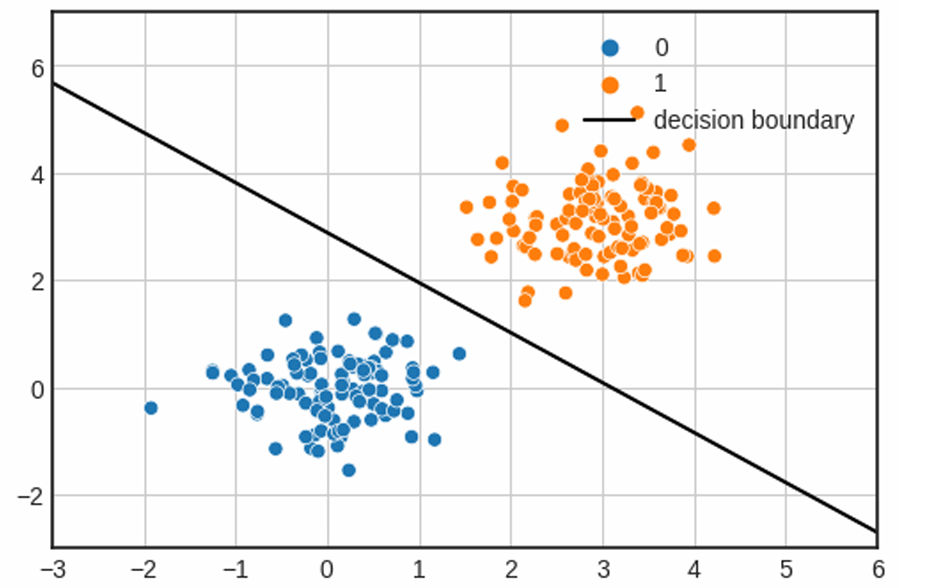
\includegraphics[width=0.7\textwidth]{./images/decision_boundary.png}
	\caption{Decision boundary del percettrone in 2D. I punti arancioni sono classificati come 1, quelli blu come 0 e la retta al centro è la \emph{decision boundary}.}
	\label{fig:decisionboundary}
\end{figure}

Questa retta, in un task di classificazione, suddivide lo spazio in due classi. In uno spazio 2D è una retta, in uno spazio 3D un piano. Lo spazio dovrà essere \textbf{linearmente separabile}.

\subsection{Processo generale di training del percettrone}
Descriviamo la procedura di training nel seguente modo:

\begin{enumerate}
	\item Inizializzazione casuale dei pesi $\vartheta_1, \dots, \vartheta_d \in \mathbb{R}$.
	\item Computa $\forall x^{(i)}$ il valore di $\hat{y}^{(i)}$.
	\item Confronta $\hat{y}^{(i)}$ con $y^{(i)}$
	\begin{itemize}
		\item Se  $\hat{y}^{(i)} = y^{(i)}$: non fare nulla.
		\item Se $\hat{y}^{(i)} \neq y^{(i)}$: vanno aggiornati i pesi. Analizziamo come modificare i pesi, in funzione dei risultati.
	\end{itemize}
	
	\item Aggiornamento dei pesi:
	
	\begin{center}
		\begin{tabular}{|c|c|c|}
			\hline
			$\hat{y}^{(i)}$ & $y^{(i)}$ & Cosa fare\\
			\hline
			0 & 0 & ok!\\
			0 & 1 & riduci i pesi.\\
			1 & 0 & aumenta i pesi.\\
			1 & 1 & ok!\\
			\hline
		\end{tabular}
	\end{center}
	
	Questo sposterà la retta in maniera opportuna, convergendo ad un risultato opportuno per il dataset di training.
\end{enumerate}

Questa descrizione generale riflette a grandi linee il processo, tuttavia è opportuno conoscere la procedura dal punto di vista matematico, che riflette poi l'implementazione effettiva.

\subsection{Implementazione del training}
L'aggiornamento dei pesi avviene nel seguente modo:
$$
\underbrace{\hat{\vartheta}_j}_\text{nuovo peso}\leftarrow \vartheta_j + ( y^{(i)} -\hat{y}^{(i)})x_j
$$

Chiaramente, il percettrone non dovrà modificare i suoi pesi se $\hat{y}^{(i)} = y^{(i)}$. Questa formula lo contempla, in quanto $y^{(i)} - \hat{y}^{(i)} = 0$: il peso non verrà aggiornato. 
Si può aggiungere un parametro $\alpha$, detto \textbf{learning rate}. Il \underline{percettrone standard non lo prevede}.

$$
\hat{\vartheta}_j \leftarrow \vartheta_j + \alpha( y^{(i)} -\hat{y}^{(i)})x_j
$$

\noindent
Scelto in maniera opportuna, potrebbe migliorare l'apprendimento e la convergenza.

\subsection{Versione di Adaline}

Una versione successiva dell'algoritmo di ricalcolo dei pesi, per stabilire con maggiore precisione di quanto incrementare o decrementare i pesi, stabilisce che

$$
\hat{\vartheta}_j \leftarrow \vartheta_j + \left( y^{(i)} - \sum_{i}\vartheta_i \cdot x_i\right)x_j
$$

\noindent
Osserviamo che, per ogni esempio $i$-esimo, l'uscita desiderata $y^{(i)}$ può assumere solo due valori, $0$ oppure $1$. Allo stesso tempo, la somma pesata 

\[
\sum_i \vartheta_i \cdot x_i
\]

\noindent
rappresenta una combinazione lineare normalizzata degli ingressi, e pertanto assume valori compresi nell'intervallo $[0,1]$.  Ne consegue che la differenza tra il valore target $y^{(i)}$ e la somma pesata non potrà che appartenere all'intervallo $[-1,1]$. In altre parole, se il neurone commette l'errore massimo possibile, questo sarà pari a $1$ in valore assoluto, cioè la distanza più grande tra un'uscita binaria ($0$ o $1$) e un valore previsto all'interno di $[0,1]$.

\section{Modelli lineari}\label{sec:modelli_lineari}
Il percettrone funziona funziona correttamente solo se i dati sono \emph{linearmente separabili}, ovvero se esiste una frontiera lineare che separa le due classi. Ad esempio, il problema AND è linearmente separabile.

\paragraph{Nota.} può essere trovato un approfondimento sulla separabilità lineare nell'appendice \ref{chap:approfondimenti_teorici}, sezione \ref{sec:separabilita_non_lineare}.

\subsection{Problema dello XOR}
Supponiamo però di voler computare lo XOR logico. Per farlo, costruiamo la tabella: 
\begin{center}
	\begin{tabular}{|c|c|c|}
		\hline
		\(x_1\) & \(x_2\) & \(XOR(x_1,x_2)\)\\
		\hline
		0 & 0 & 0\\
		0 & 1 & 1\\
		1 & 0 & 1\\
		1 & 1 & 0\\
		\hline
	\end{tabular}
\end{center}

\noindent
Il problema XOR non è linearmente separabile (immagine \ref{fig:xor-schema}): i quattro punti \((0,0),(1,0),(0,1),(1,1)\) con etichetta di uscita \(0,1,1,0\) non possono essere separati da una singola frontiera lineare. Un percettrone (che produce solo confini di decisione lineari) non riesce quindi a risolverlo.

\begin{figure}[htbp]
	\centering
	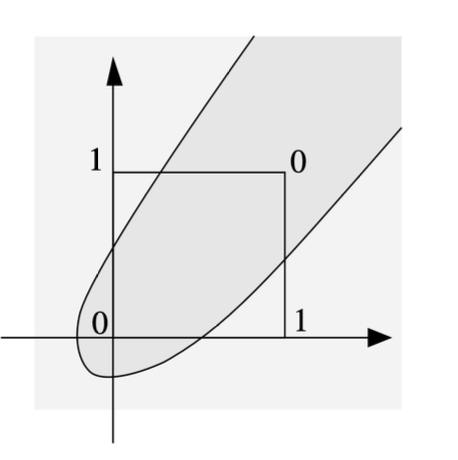
\includegraphics[width=.55\linewidth]{images/xor-schema.jpg}
	\caption{Schema del problema XOR: i vertici \((0,1)\) e \((1,0)\) appartengono alla classe \(1\), \((0,0)\) e \((1,1)\) alla classe \(0\). Nessuna frontiera lineare può separare le classi; è necessaria una frontiera non lineare (ottenibile con uno strato nascosto).}
	\label{fig:xor-schema}
\end{figure}

\paragraph{Dimostrazione della non-linearità dello XOR.} Assumendo la tabella di verità dello XOR e un percettrone con pesi \(\vartheta_1,\vartheta_2\) e soglia \(\vartheta_0\), le condizioni di attivazione diventano

\[
\begin{aligned}
	&1\cdot \vartheta_1 + 0\cdot \vartheta_2 > \vartheta_0,\\
	&1\cdot \vartheta_1 + 1\cdot \vartheta_2 < \vartheta_0,\\
	&0\cdot \vartheta_1 + 1\cdot \vartheta_2 > \vartheta_0,\\
	&0\cdot \vartheta_1 + 0\cdot \vartheta_2 < \vartheta_0.
\end{aligned}
\]

Da cui si ottiene
\[
2\,\vartheta_0 < \vartheta_1 + \vartheta_2 < \vartheta_0,
\]
ovvero una contraddizione: non esiste configurazione dei parametri di un singolo percettrone che risolva XOR.


\subsection{Rete di percettroni} 
La soluzione consiste nell'usare una \emph{rete di percettroni} (uno strato nascosto) che trasformi lo spazio in modo da rendere il problema linearmente separabile all'uscita. 

Un esempio minimale è:
\[
\begin{aligned}
	&f_1(x_1,x_2) = [\,x_1 - x_2 \ge 0.5\,],\\
	&f_2(x_1,x_2) = [\,x_2 - x_1 \ge 0.5\,],\\
	&f_3\big(f_1,f_2\big) = [\,1\cdot f_1 + 1\cdot f_2 \ge 0.5\,],
\end{aligned}
\]
dove \([\cdot]\) indica una funzione soglia (vale \(1\) se la condizione è vera, \(0\) altrimenti). Le funzioni \(f_1\) e \(f_2\) realizzano una trasformazione non lineare degli input; nello spazio così trasformato l'uscita \(f_3\) è ottenuta tramite una semplice soglia lineare.

Infine, sebbene reti di percettroni possano risolvere $XOR$, l'algoritmo di apprendimento del singolo percettrone non è direttamente applicabile a reti multistrato; storicamente ciò contribuì al primo \emph{AI winter} e la situazione migliorò con la formalizzazione della \emph{retropropagazione} (\emph{backpropagation}). 

\paragraph{Caso studio.}
Consideriamo ora la rete mostrata in figura \ref{fig:nn-xor}, con pesi esplicitamente indicati. I nodi $a_1$ e $a_2$ costituiscono lo strato nascosto, mentre $a_3$ rappresenta il neurone di uscita. Il nodo costante $1$ implementa il bias (termine di soglia) tramite pesi negativi.

\begin{figure}[tbph]
	\centering
	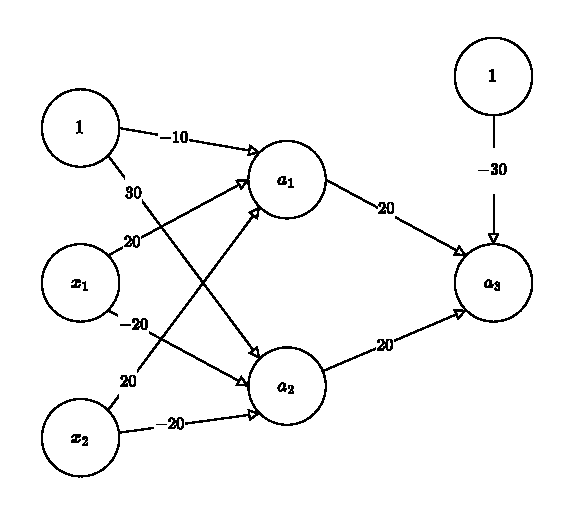
\includegraphics[width=0.7\linewidth]{images/neural-net-xor}
	\caption{Rete di percettroni per computare lo $XOR$}
	\label{fig:nn-xor}
\end{figure}

I neuroni nascosti sono definiti da:
\[
a_1 = \mathbf{1}\{-10\cdot 1 + 20x_1 + 20x_2 \ge 0\},
\]
\[
a_2 = \mathbf{1}\{30\cdot 1 -20x_1 -20x_2 \ge 0\}.
\]

Il neurone di uscita è:
\[
a_3 = \mathbf{1}\{-30\cdot 1 + 20a_1 + 20a_2 \ge 0\}.
\]

Verifichiamo ora i quattro casi possibili di $(x_1,x_2)$:

\begin{itemize}
\item $(0,0)$:  
$a_1=0$, $a_2=1$ $\Rightarrow$ $a_3=0$.
\item $(0,1)$:  
$a_1=1$, $a_2=0$ $\Rightarrow$ $a_3=1$.
\item $(1,0)$:  
$a_1=1$, $a_2=0$ $\Rightarrow$ $a_3=1$.
\item $(1,1)$:  
$a_1=0$, $a_2=0$ $\Rightarrow$ $a_3=0$.
\end{itemize}

Si ottiene quindi esattamente la tabella di verità dello XOR. 

Questo esempio mostra in modo concreto come uno strato nascosto realizzi una trasformazione non lineare dello spazio di input: i neuroni $a_1$ e $a_2$ costruiscono due regioni linearmente separabili, che il neurone finale combina linearmente per ottenere una frontiera di decisione non lineare nello spazio originale.


\section*{Riferimenti}
Il materiale visto per questo capitolo comprende:
\begin{itemize}
    \item Materiale visto a lezione.
    \item Note del prof. Antonino Furnari.
    \item Materiale sul percettrone dal libro \citetitle{Rojas1996} \cite{Rojas1996}.
\end{itemize}